%%%%%%%%%%%%%%%%%%%%%%%%%%%%%%%%%%%%%%%%%
% Beamer Presentation
% LaTeX Template
% Version 1.0 (10/11/12)
%
% This template has been downloaded from:
% http://www.LaTeXTemplates.com
%
% License:
% CC BY-NC-SA 3.0 (http://creativecommons.org/licenses/by-nc-sa/3.0/)
%
%%%%%%%%%%%%%%%%%%%%%%%%%%%%%%%%%%%%%%%%%

%----------------------------------------------------------------------------------------
%	PACKAGES AND THEMES
%----------------------------------------------------------------------------------------

\documentclass{beamer}

\mode<presentation> {

% The Beamer class comes with a number of default slide themes
% which change the colors and layouts of slides. Below this is a list
% of all the themes, uncomment each in turn to see what they look like.

%\usetheme{default}
%\usetheme{AnnArbor}
%\usetheme{Antibes}
%\usetheme{Bergen}
%\usetheme{Berkeley}
%\usetheme{Berlin}
%\usetheme{Boadilla}
%\usetheme{CambridgeUS}
%\usetheme{Copenhagen}
%\usetheme{Darmstadt}
%\usetheme{Dresden}
%\usetheme{Frankfurt}
%\usetheme{Goettingen}
%\usetheme{Hannover}
%\usetheme{Ilmenau}
%\usetheme{JuanLesPins}
\usetheme{Luebeck}
%\usetheme{Madrid}
%\usetheme{Malmoe}
%\usetheme{Marburg}
%\usetheme{Montpellier}
%\usetheme{PaloAlto}
%\usetheme{Pittsburgh}
%\usetheme{Rochester}
%\usetheme{Singapore}
%\usetheme{Szeged}
%\usetheme{Warsaw}

% As well as themes, the Beamer class has a number of color themes
% for any slide theme. Uncomment each of these in turn to see how it
% changes the colors of your current slide theme.

%\usecolortheme{albatross}
%\usecolortheme{beaver}
%\usecolortheme{beetle}
%\usecolortheme{crane}
%\usecolortheme{dolphin}
%\usecolortheme{dove}
%\usecolortheme{fly}
%\usecolortheme{lily} % das ist gut
%\usecolortheme{orchid}
%\usecolortheme{rose}
%\usecolortheme{seagull}
%\usecolortheme{seahorse}
%\usecolortheme{whale}
%\usecolortheme{wolverine}

%\setbeamertemplate{footline} % To remove the footer line in all slides uncomment this line
\setbeamertemplate{footline}[page number] % To replace the footer line in all slides with a simple slide count uncomment this line

\setbeamertemplate{navigation symbols}{} % To remove the navigation symbols from the bottom of all slides uncomment this line
}

\usepackage{graphicx} % Allows including images
	\graphicspath{{PDF/},{./}}
	\DeclareGraphicsExtensions{.pdf,.png}
\usepackage{booktabs} % Allows the use of \toprule, \midrule and \bottomrule in tables
\usepackage{url}

%----------------------------------------------------------------------------------------
%	TITLE PAGE
%----------------------------------------------------------------------------------------

\title[StreamGraph]{StreamGraph} % The short title appears at the bottom of every slide, the full title is only on the title page

\author{Florian Ziesche, Jakob Karge and Boris Graf} % Your name
\institute[TUB] % Your institution as it will appear on the bottom of every slide, may be shorthand to save space
{
Technische Universit\"at Berlin\\ % Your institution for the title page
}
\date{\today} % Date, can be changed to a custom date

\begin{document}

\begin{frame}
\titlepage % Print the title page as the first slide
\begin{figure}[H]
		\centering
		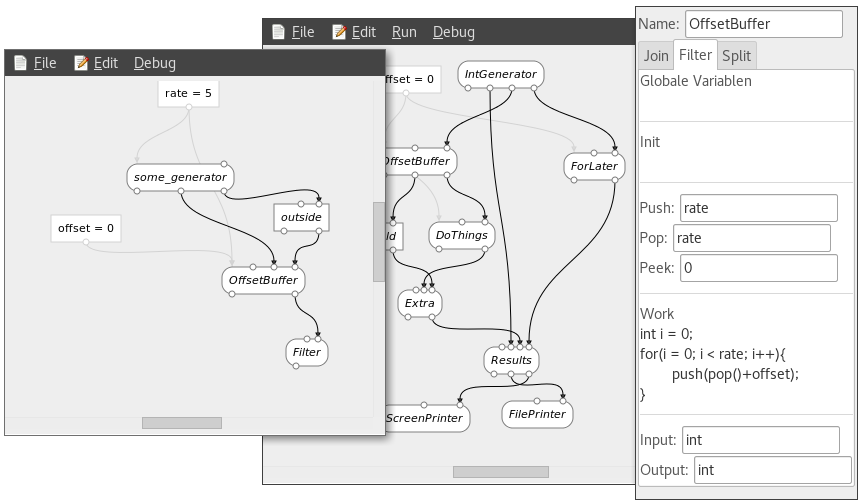
\includegraphics[width=0.7\textwidth]{streamgraph}
	\end{figure}
\end{frame}

\begin{frame}
\frametitle{Overview} % Table of contents slide, comment this block out to remove it
\tableofcontents % Throughout your presentation, if you choose to use \section{} and \subsection{} commands, these will automatically be printed on this slide as an overview of your presentation
\end{frame}

%----------------------------------------------------------------------------------------
%	PRESENTATION SLIDES
%----------------------------------------------------------------------------------------

%------------------------------------------------
\section{Introduction} % Sections can be created in order to organize your presentation into discrete blocks, all sections and subsections are automatically printed in the table of contents as an overview of the talk
%------------------------------------------------
\subsection{Idea \& Goals}
% Jakob
\begin{frame}
\frametitle{Idea \& Goals}
\begin{itemize}
	\item Visualize parallel programming
	\item Graphical layer on top of a textual language
\end{itemize}
\begin{itemize}
	\item StreamIt: subset representation
\end{itemize}
\end{frame}

\subsection{SreamIt}
% Florian
\begin{frame}
\frametitle{StreamIt}
	\begin{itemize}
		\item Developed for streaming applications
		\item Pipeline-based structure
	\end{itemize}
	\begin{block}{Base constructs}
		\begin{itemize}
			\item Filter: "The Workhorse of StreamIt"; \textit{work}-, \textit{init}-functions 
			\item Pipeline: linear succession of StreamIt constructs
			\item Split-Join: creating parallel paths
			\begin{itemize}
				\item Split: split single data stream into multiple data streams
				\item Join: join previously splitted streams together
			\end{itemize}
			% \item FeedbackLoop
		\end{itemize}
	\end{block}
	For further information on StreamIt see \cite{streamIt}.
\end{frame}
%------------------------------------------------

\begin{frame}
\frametitle{Parallelism in StreamIt}
	\begin{block}{Split-Join}
		%Data-parallelism
		Splitting (or duplicating) of data:\\
		\begin{itemize}
			\item Paths independent between \textit{split} and \textit{join}
		\end{itemize}
		As result paths may be processed in parallel
	\end{block}
	\begin{block}{Pipeline}
		Continuous data stream through filters:\\
		\begin{itemize}
			\item \textit{Work}-functions are constantly recalculated.
			\item Filters can be processed independently.
		\end{itemize}
		Therefore filters in pipelines can be parallelised.
	\end{block}
\end{frame}

%------------------------------------------------
\subsection{StreamGraph GUI}
% Boris
\begin{frame}
\frametitle{StreamGraph GUI}
	\begin{itemize}
		\item Minimalistic and clear design
		\item Mouse control via pop-up menus
		\item Intuitive control
	\end{itemize}
	\begin{block}{Elements}
		\begin{itemize}
			\item Menu bar
			\item Working surface
			\item Notification bar
			\item Property window
		\end{itemize}
	\end{block}
\end{frame}

\begin{frame}
\frametitle{StreamGraph GUI}
	Visual abstractions of StreamIt toplogy
	\begin{columns}[c]
		\begin{column}{0.48\textwidth}
			\begin{itemize}	
				\item Split \& join integrated into filters
				\item Implicit pipelines
			\end{itemize}
		\end{column}
		\hfill
		\begin{column}{0.48\textwidth}
			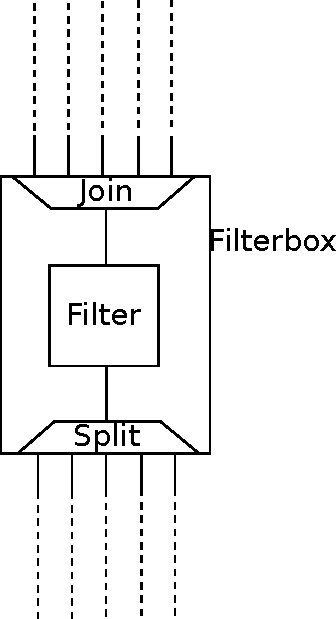
\includegraphics[width=0.6\textwidth]{FilterBoxGraphic}
			\label{fig_filterAbstraction}		
		\end{column}
	\end{columns}		
\end{frame}


%------------------------------------------------
\section{Demo}
\begin{frame}
\frametitle{Demo}
	\textbf{DEMO}: \texttt{demoPower.str}
	\begin{figure}[h]
		\centering
		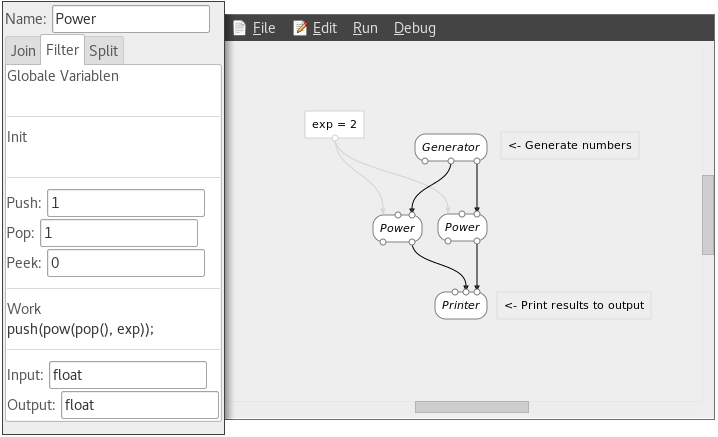
\includegraphics[width=0.8\textwidth]{demoPower}
		\label{fig_demoPower}
	\end{figure}
\end{frame}


%------------------------------------------------
\section{Backend}

%------------------------------------------------
\subsection{Framework}
% Boris
\begin{frame}
\frametitle{StreamGraph View}
 \begin{itemize}
 	\item Based on Gtk2::Ex::MindMapView \cite{GTK2EXMindMapView}
	\item Gnome Canvas used as engine
	\item Item $\rightarrow$ border $\rightarrow$ content
	\item Handle keyboard and mouse events
	\item Many other changes
 \end{itemize}
\end{frame}


%------------------------------------------------
\subsection{Model}
% Jakob
\begin{frame}
\frametitle{Model}
Program structures modeled in two ways:
\begin{block}{Graphical: \textit{Node}}
	\begin{itemize}
		\item Node types (\textit{Filter, Subgraph, Parameter, Comment})
		\item Factory
	\end{itemize}
\end{block}
% should that be here?
% maybe add it to Code Generation Slides?
\begin{block}{Textual: \textit{CodeObject}}
	\begin{itemize}
		\item StreamIt types (\textit{Pipeline, Splitjoin, Parameter})
		\item \textit{CodeObject}s derived from \textit{Node}s
	\end{itemize}
\end{block}
\end{frame}

\subsection{Graph Transformation}
% TODO: pictures for every step
\begin{frame}
\frametitle{Graph Transformation}
	\begin{columns}[c]
		\begin{column}{0.48\textwidth}
			\begin{itemize}
				\item Load subgraphs
				\item Add void sources and -sinks
				\item Add identities for empty pipelines
				\item Test for graph errors %throughout the above and leave invalid partial graphs alone
			\end{itemize}
		\end{column}
		\hfill
		\begin{column}{0.48\textwidth}
			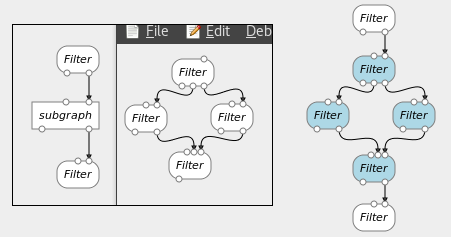
\includegraphics[width=1.035\textwidth]{subgraph_before_after}\\
			\vspace{1.1mm}
			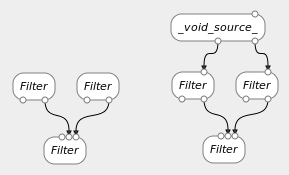
\includegraphics[width=0.53\textwidth]{voidend_before_after} ~
			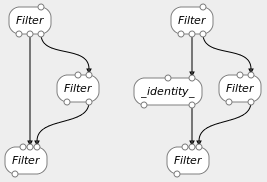
\includegraphics[width=0.47\textwidth]{identity_before_after}
		\end{column}
	\end{columns}
\end{frame}

%------------------------------------------------
\subsection{Code Generation}
% Florian
\begin{frame}
\frametitle{Code Generation}
	\begin{block}{General procedure}
		\begin{itemize}
			\item Generate code for all filters
			\item Build pipeline-based structure
			\item Generate code for topology in recursive manner
		\end{itemize}
	\end{block}
	\begin{block}{Filter generation}
		\begin{itemize}
			\item Make name unique
			\item Get parameters
			\item Build \textit{init}- and \textit{work}- function
		\end{itemize}
	\end{block}
\end{frame}
%------------------------------------------------

\begin{frame}
\frametitle{StreamIt pipeline-based structure}
	\begin{figure}[h]
		\centering
		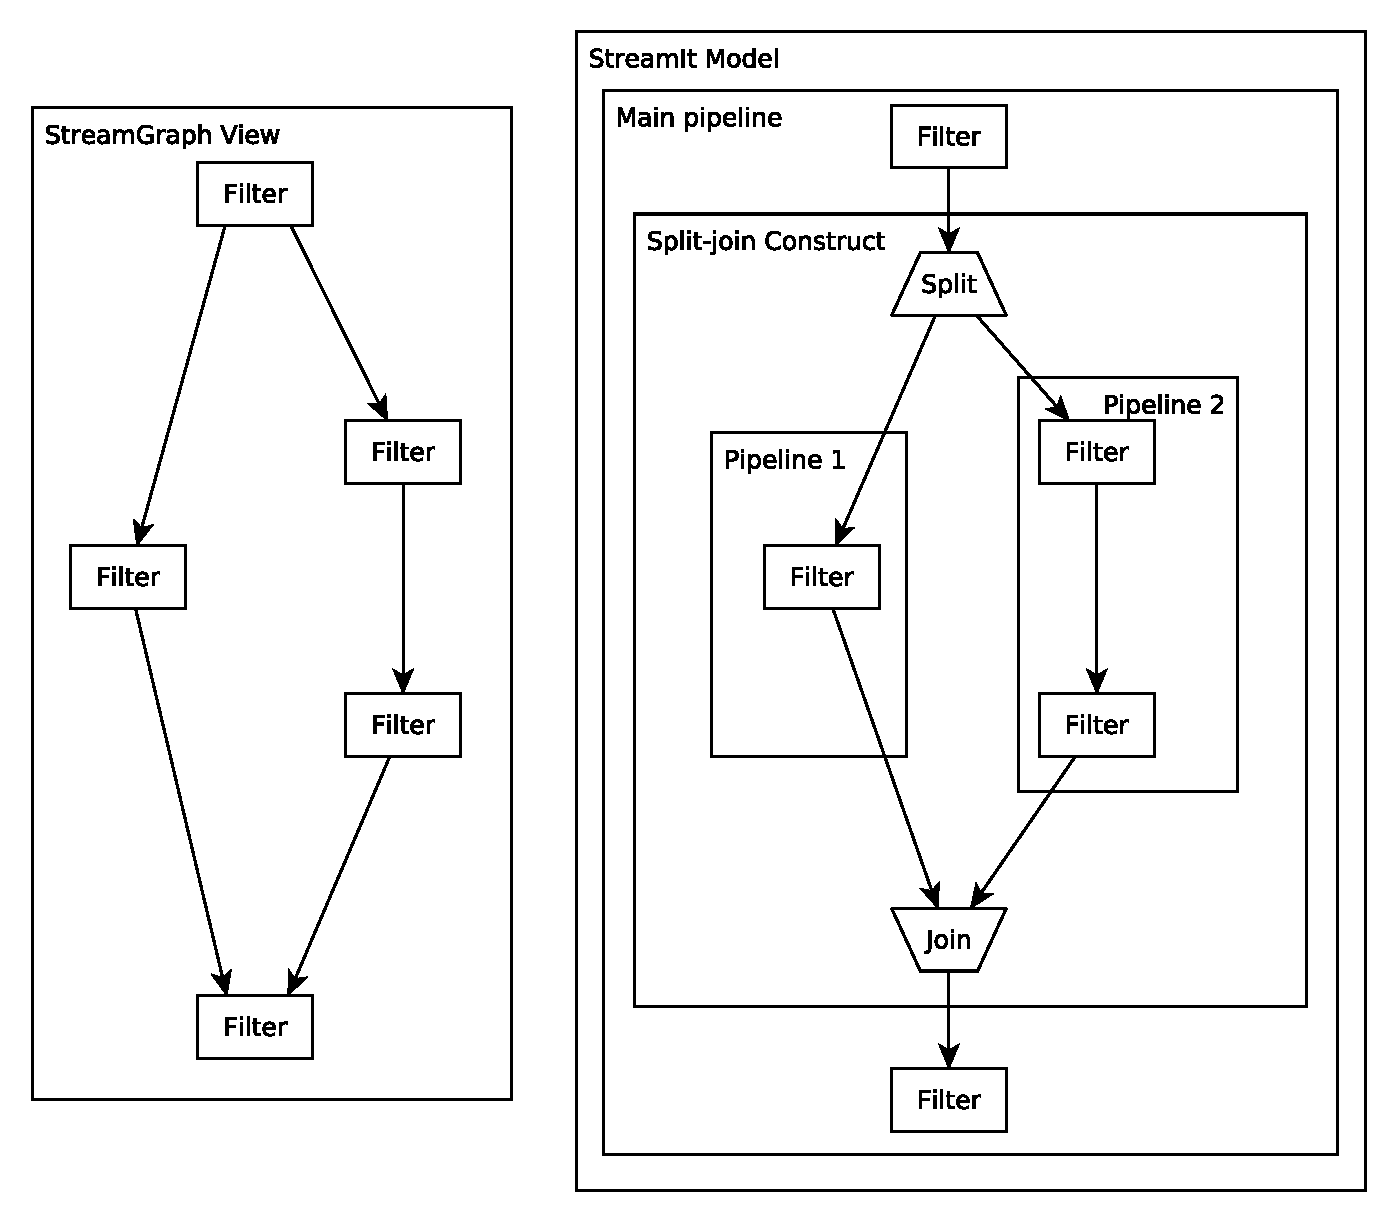
\includegraphics[width=\textwidth]{StreamGraphToStreamIt}
		\label{fig_StreamGraph_To_StreamIt}
	\end{figure}
\end{frame}


%------------------------------------------------
\begin{frame}
\frametitle{Code Generation}
	\begin{block}{Building the structure}
		\begin{itemize}
			\item Begin with pipeline (main)
			\item If split is detected start building of split-join\\
				\quad Build a pipeline for every Path.
			\item Continue with generation of pipeline.
		\end{itemize}
		Indirect recursive method guarantees StreamIt-type hierarchical structure
	\end{block}
	Get the code by generating from inside out.
\end{frame}

%------------------------------------------------
\section{Conclusion}
% ???

%------------------------------------------------
\subsection{Results}
\begin{frame}
\frametitle{Results}
	\begin{itemize}
		\item Working prototype
		\item Limited StreamIt representation
		\item Complete toolchain from "empty" to "running"
	\end{itemize}
\end{frame}

%------------------------------------------------
\subsection{Improvements \& Future}
\begin{frame}
\frametitle{Improvements}
	\begin{itemize}
		\item Ordered splitjoin (currently only commutative use of results)
		\item More StreamIt constructs (e.g. message passing, feedback-loop)
		\item UI
		\begin{itemize}
			\item Group-to-subgraph
			\item In-graph error highlighting
			\item Data visualization
			\item ...
		\end{itemize}
		\item More automatic compatability
		\item StreamIt+Java1.5+Perl-packages auto setup
		\item Code quality \& style
	\end{itemize}
\end{frame}

\begin{frame}
\frametitle{Future}
Possible research and development directions
	\begin{itemize}
		\item Different background language
		\item More general graphical environment
	\end{itemize}
\end{frame}


%------------------------------------------------
\section*{Bibliography}
\begin{frame}
\frametitle{Bibliography}
\footnotesize{
	\begin{thebibliography}{99} % Beamer does not support BibTeX so references must be inserted manually as below
	\bibitem{streamIt}
		William~Thies, Michael~Karczmarek, and Saman~Amarasinghe, \emph{StreamIt: A Language for Streaming Applications},
		\hskip 1em plus
		0.5em minus 0.4em\relax Laboratory for Computer Science, Massachusetts Institute of Technology, Cambridge, MA 02139.
	\bibitem{GTK2EXMindMapView}
		\url{http://search.cpan.org/~hemlock/Gtk2-Ex-MindMapView-0.000001/lib/Gtk2/Ex/MindMapView.pm}

	\end{thebibliography}
}
\end{frame}

%----------------------------------------------------------------------------------------

\end{document}
